\documentclass[11pt]{article}

\usepackage[margin=1in]{geometry}
\usepackage{amsmath,amssymb,amsthm,mathtools}
\usepackage{booktabs}
\usepackage{enumitem}
\usepackage{graphicx}
\usepackage{tikz}
\usetikzlibrary{arrows.meta,positioning,shapes.geometric,fit}
\usepackage[colorlinks=true,linkcolor=blue,citecolor=blue,urlcolor=blue]{hyperref}
\usepackage{xcolor}

\newtheorem{theorem}{Theorem}
\newtheorem{proposition}{Proposition}
\newtheorem{corollary}{Corollary}
\newtheorem{assumption}{Assumption}
\newtheorem{remark}{Remark}

\newcommand{\E}{\mathbb{E}}
\newcommand{\1}{\mathbf{1}}
\newcommand{\calF}{\mathcal{F}}
\newcommand{\calG}{\mathcal{G}}
\newcommand{\R}{\mathbb{R}}
\newcommand{\Yhat}{\widehat Y}
\newcommand{\ellhat}{\widehat\ell}
\newcommand{\Hhat}{\widehat H}
\newcommand{\eps}{\epsilon}

\title{Audited Online Dual-Price PAC Labeling\\
\large A Partial-Feedback Extension of PAC Labeling with Finite-Horizon Error Control}
\author{Draft proposal}
\date{\today}

\begin{document}
\maketitle

\begin{abstract}
We study an online extension of probably approximately correct (PAC) labeling in which inputs arrive sequentially, labeling decisions are irrevocable, and expert labels are costly. A direct adaptive-conformal-style update is not valid in this setting because the realized loss of an AI-labeled point is not observed unless the expert label is revealed. We therefore introduce an audited online dual-price algorithm. The algorithm maintains a scalar price of error, uses that price to decide whether to route an input to a cheap AI source or defer to the expert, and performs randomized audits of AI-labeled points to obtain intermittent feedback. The audit correction is an inverse-observation-probability estimator, analogous to intermittent online conformal prediction. We give finite-horizon high-probability error control under explicit assumptions. The result is deliberately modest: it controls realized labeling error, but does not claim cost optimality relative to an offline LP without additional stochastic-arrival assumptions.
\end{abstract}

\section{Setup}

We consider a streaming data-curation problem. At each round $t=1,\ldots,T$, an input $X_t$ arrives and must be assigned a final label $\widetilde Y_t$. There are $k$ cheap non-expert labeling sources. Source $j\in[k]$ provides a predicted label
\[
\Yhat_t^{(j)}
\]
at cost $c_j\ge 0$. Querying an expert reveals the true label $Y_t$ at cost $c_{\mathrm{expert}}>0$. The expert label is treated as correct. The loss is bounded,
\[
0\le \ell(Y_t,\Yhat_t^{(j)})\le 1.
\]
The target is a finite-horizon average labeling error constraint
\[
\frac{1}{T}\sum_{t=1}^T \ell(Y_t,\widetilde Y_t)\le \eps,
\]
with high probability over the algorithm's audit randomness.

The main obstacle is partial feedback. If the algorithm uses an AI label and does not query the expert, then $Y_t$ is not observed and the realized loss $\ell(Y_t,\widetilde Y_t)$ is unavailable. Thus the full-feedback adaptive-conformal update cannot be applied directly. We resolve this by adding randomized audits: after choosing to use an AI label, the algorithm independently queries the expert with known probability $p_t\in[p_{\min},1]$. If audited, the expert label is observed. This creates intermittent feedback and allows inverse-probability correction, as in intermittent online conformal prediction.

\paragraph{Two distinct expert-query roles.}
We separate final-label deferral from auditing. Let
\[
D_t=\1\{\text{the algorithm defers to the expert as the final label}\}
\]
and
\[
A_t=\1\{\text{an AI-labeled point is randomly audited}\}.
\]
If $D_t=1$, then $\widetilde Y_t=Y_t$ and the final loss is zero. If $D_t=0$, the algorithm initially uses an AI label. It may nevertheless audit the point. In the audit-and-correct version used below, an audited AI-labeled point is corrected to the expert label in the final dataset, while the counterfactual AI error is still used for updating the price.

\begin{figure}[t]
\centering
\resizebox{\linewidth}{!}{%
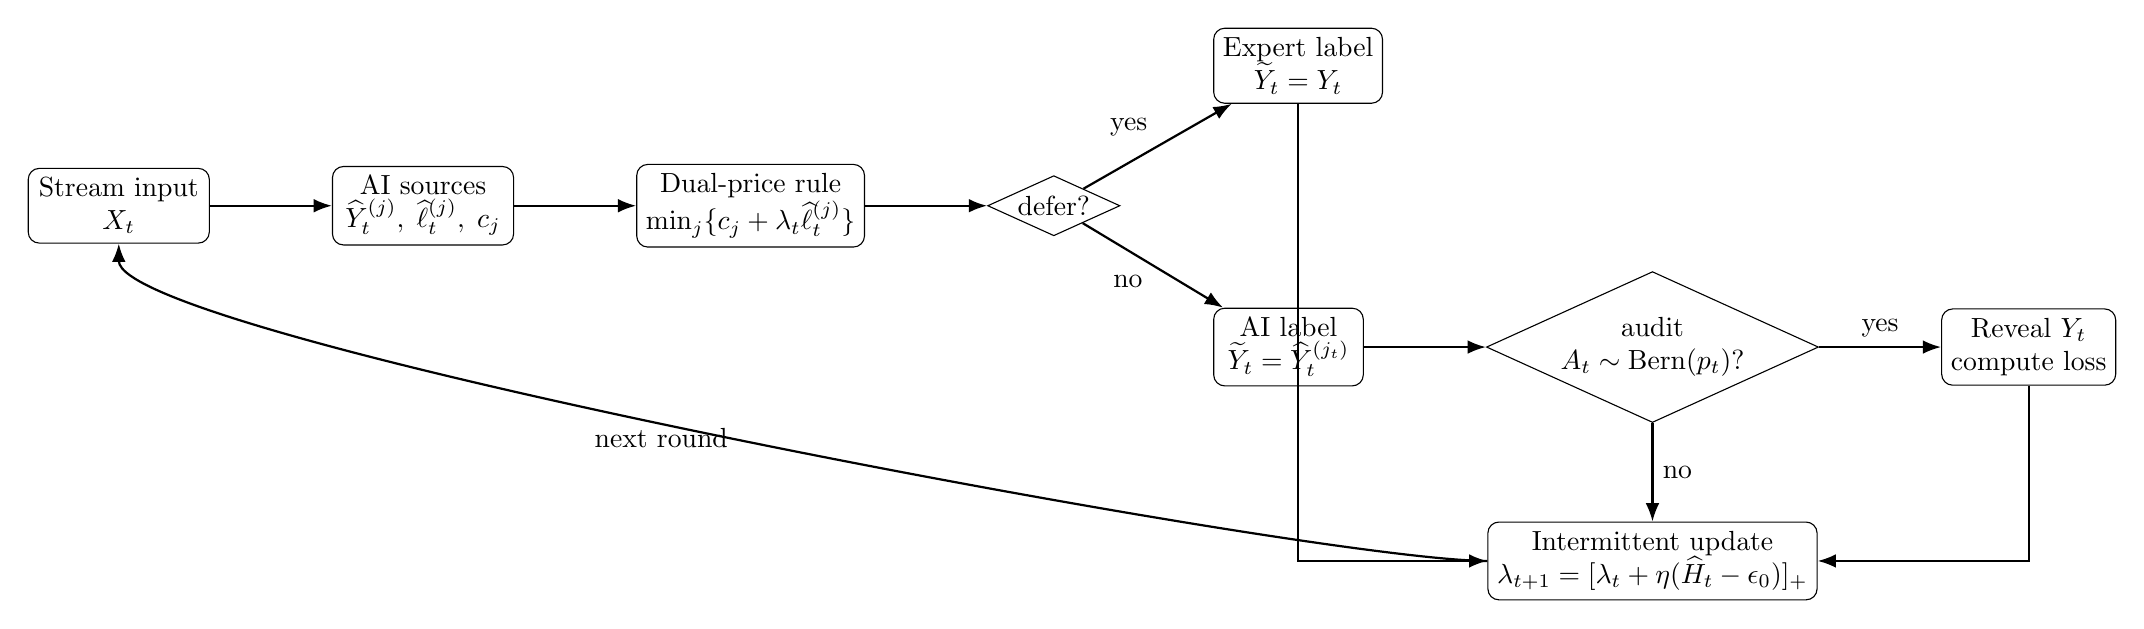
\begin{tikzpicture}[
  node distance=1.55cm,
  block/.style={draw, rounded corners, align=center, minimum height=0.9cm, minimum width=2.3cm},
  smallblock/.style={draw, rounded corners, align=center, minimum height=0.75cm, minimum width=1.9cm},
  decision/.style={draw, diamond, aspect=2.2, align=center, inner sep=1pt},
  arrow/.style={-Latex, thick}
]

\node[block] (input) {Stream input\\$X_t$};
\node[block, right=of input] (sources) {AI sources\\$\Yhat_t^{(j)},\;\ellhat_t^{(j)},\;c_j$};
\node[block, right=of sources] (price) {Dual-price rule\\$\min_j\{c_j+\lambda_t\ellhat_t^{(j)}\}$};
\node[decision, right=of price] (defer) {defer?};

\node[smallblock, above right=1.1cm and 1.6cm of defer] (expert) {Expert label\\$\widetilde Y_t=Y_t$};
\node[smallblock, below right=1.1cm and 1.6cm of defer] (ai) {AI label\\$\widetilde Y_t=\Yhat_t^{(j_t)}$};
\node[decision, right=of ai] (audit) {audit\\$A_t\sim\mathrm{Bern}(p_t)$?};
\node[smallblock, right=of audit] (reveal) {Reveal $Y_t$\\compute loss};
\node[block, below=1.25cm of audit] (update) {Intermittent update\\$\lambda_{t+1}=[\lambda_t+\eta(\Hhat_t-\epsilon_0)]_+$};

\draw[arrow] (input) -- (sources);
\draw[arrow] (sources) -- (price);
\draw[arrow] (price) -- (defer);
\draw[arrow] (defer) -- node[above left] {yes} (expert);
\draw[arrow] (defer) -- node[below left] {no} (ai);
\draw[arrow] (ai) -- (audit);
\draw[arrow] (audit) -- node[above] {yes} (reveal);
\draw[arrow] (reveal) |- (update);
\draw[arrow] (expert) |- (update);
\draw[arrow] (audit) -- node[right] {no} (update);
\draw[arrow] (update.west) .. controls +(left:2.2cm) and +(down:1.2cm) .. node[left] {next round} (input.south);
\end{tikzpicture}%
}
\caption{Online audited PAC labeling. The dual price $\lambda_t$ decides whether the current point is labeled by a cheap AI source or by the expert. AI-labeled points are randomly audited with known probability $p_t$. Audited labels provide intermittent feedback for the price update.}
\label{fig:setup}
\end{figure}

\section{Algorithm}

The algorithm maintains a scalar error price $\lambda_t\ge 0$. A larger $\lambda_t$ makes AI errors more expensive and therefore causes more deferral to the expert.

At round $t$, suppose each source has a predictable loss estimate
\[
\ellhat_t^{(j)}=\ellhat^{(j)}(X_t)\in[\rho,1]
\]
for some fixed $\rho>0$. The estimate may be produced by a warm-up calibrator, by multicalibration, by isotonic regression, or by any online calibrator using only past expert/audit labels. The theorem below does not require this estimate to be accurate; it only needs to be predictable and lower bounded.

\paragraph{Decision rule.}
Choose
\[
j_t^\star\in\arg\min_{j\in[k]}\{c_j+\lambda_t\ellhat_t^{(j)}\}.
\]
If
\[
c_{j_t^\star}+\lambda_t\ellhat_t^{(j_t^\star)}\ge c_{\mathrm{expert}},
\]
then defer to the expert:
\[
D_t=1,\qquad \widetilde Y_t=Y_t,\qquad \Hhat_t=0.
\]
Otherwise, use the AI source $j_t^\star$:
\[
D_t=0,\qquad \widetilde Y_t=\Yhat_t^{(j_t^\star)}.
\]
Then draw an independent audit variable
\[
A_t\sim \mathrm{Bernoulli}(p_t),\qquad p_t\in[p_{\min},1].
\]
If $A_t=1$, query the expert, observe $Y_t$, and optionally correct the final dataset label by setting $\widetilde Y_t=Y_t$. For updating the price, use the importance-weighted counterfactual AI loss
\[
\Hhat_t=(1-D_t)\frac{A_t}{p_t}\ell(Y_t,\Yhat_t^{(j_t^\star)}).
\]
Finally update
\begin{equation}
\lambda_{t+1}=\left[\lambda_t+\eta(\Hhat_t-\epsilon_0)\right]_+,
\label{eq:update}
\end{equation}
where $\eta>0$ is a step size and $\epsilon_0\le \epsilon$ is an internal target used to leave room for finite-sample audit noise.

\begin{center}
\fbox{%
\begin{minipage}{0.93\linewidth}
\textbf{Algorithm 1: Audited Online Dual-Price PAC Labeling}
\begin{enumerate}[leftmargin=1.5em]
\item Initialize $\lambda_1\ge 0$, step size $\eta>0$, internal target $\epsilon_0\in[0,\epsilon]$.
\item For $t=1,\ldots,T$:
  \begin{enumerate}[leftmargin=1.5em]
  \item Observe $X_t$, cheap labels $\Yhat_t^{(j)}$, costs $c_j$, and predictable estimates $\ellhat_t^{(j)}$.
  \item Set $j_t^\star\in\arg\min_j\{c_j+\lambda_t\ellhat_t^{(j)}\}$.
  \item If $c_{j_t^\star}+\lambda_t\ellhat_t^{(j_t^\star)}\ge c_{\mathrm{expert}}$, defer: query expert, output $\widetilde Y_t=Y_t$, set $\Hhat_t=0$.
  \item Otherwise, output the AI label $\Yhat_t^{(j_t^\star)}$. Draw $A_t\sim\mathrm{Bernoulli}(p_t)$. If $A_t=1$, query expert, optionally correct $\widetilde Y_t=Y_t$, and set $\Hhat_t=(A_t/p_t)\ell(Y_t,\Yhat_t^{(j_t^\star)})$. If $A_t=0$, set $\Hhat_t=0$.
  \item Update $\lambda_{t+1}=[\lambda_t+\eta(\Hhat_t-
\epsilon_0)]_+$.
  \end{enumerate}
\end{enumerate}
\end{minipage}}
\end{center}

\section{Theoretical Results}

We give finite-horizon error control. The result is distribution-free with respect to the data sequence; the probability is only over audit randomness. It does not claim cost optimality.

\subsection{Assumptions}

\begin{assumption}[Bounded loss]
For all $t$ and $j$,
\[
0\le \ell(Y_t,\Yhat_t^{(j)})\le 1.
\]
\end{assumption}

\begin{assumption}[Predictability]
Before the audit draw $A_t$, the quantities $X_t$, $\Yhat_t^{(j)}$, $\ellhat_t^{(j)}$, $p_t$, $D_t$, and $j_t^\star$ are measurable with respect to the available history and the current input. The data sequence may be arbitrary or adaptive to past interactions.
\end{assumption}

\begin{assumption}[Random audit]
If $D_t=0$, then
\[
A_t\mid \calG_t\sim\mathrm{Bernoulli}(p_t),\qquad p_t\in[p_{\min},1],
\]
where $\calG_t$ denotes the sigma-field after the decision has been made and before the audit draw. Mathematically $\calG_t$ may include the latent $Y_t$; the learner need not observe it. The audit draw is conditionally independent of all other randomness given $\calG_t$.
\end{assumption}

\begin{assumption}[Loss-estimate floor]
For some $\rho>0$,
\[
\ellhat_t^{(j)}\in[\rho,1]
\]
for all $t,j$.
\end{assumption}

\begin{assumption}[Correct expert]
Expert labels are correct. Deferring to the expert incurs zero final labeling loss.
\end{assumption}

\subsection{Statements}

Define the counterfactual AI-decision loss
\[
H_t=(1-D_t)\ell(Y_t,\Yhat_t^{(j_t^\star)}).
\]
This is the loss that would be incurred by the AI decision before audit correction. The actual final loss after audit-and-correct is
\[
G_t=\ell(Y_t,\widetilde Y_t),
\]
and satisfies $G_t\le H_t$.

\begin{proposition}[Unbiased audited loss estimate]
Under Assumptions 1--3,
\[
\E[\Hhat_t\mid\calG_t]=H_t.
\]
\end{proposition}

\begin{theorem}[Finite-horizon high-probability error control]
Let
\[
c_{\min}=\min_{j\in[k]}c_j,
\qquad
\lambda_{\mathrm{def}}=\frac{(c_{\mathrm{expert}}-c_{\min})_+}{\rho}.
\]
Run Algorithm 1 with constant step size $\eta>0$ and internal target $\epsilon_0\in[0,\epsilon]$. Define
\[
\Lambda=\max\left\{\lambda_1,\lambda_{\mathrm{def}}+\frac{\eta}{p_{\min}}\right\}.
\]
Then, for any fixed horizon $T$ and any $\delta\in(0,1)$, with probability at least $1-\delta$ over the audit randomness,
\begin{equation}
\frac{1}{T}\sum_{t=1}^T H_t
\le
\epsilon_0+\frac{\Lambda}{\eta T}+\frac{1}{p_{\min}}\sqrt{\frac{2\log(1/\delta)}{T}}.
\label{eq:Hbound}
\end{equation}
Consequently, if audited AI labels are corrected to expert labels in the final dataset, then
\begin{equation}
\frac{1}{T}\sum_{t=1}^T G_t
\le
\epsilon_0+\frac{\Lambda}{\eta T}+\frac{1}{p_{\min}}\sqrt{\frac{2\log(1/\delta)}{T}}
\label{eq:Gbound}
\end{equation}
with probability at least $1-\delta$.
\end{theorem}

\begin{corollary}[PAC-style tuning]
Suppose the desired tolerance is $\epsilon$. If
\[
\epsilon_0
=
\epsilon-\frac{\Lambda}{\eta T}-\frac{1}{p_{\min}}\sqrt{\frac{2\log(1/\delta)}{T}}
\]
is positive, then Algorithm 1 satisfies
\[
\frac{1}{T}\sum_{t=1}^T \ell(Y_t,\widetilde Y_t)\le \epsilon
\]
with probability at least $1-\delta$. With $\eta\asymp T^{-1/2}$ and constant $p_{\min}$, the slack is $O(T^{-1/2})$.
\end{corollary}

\begin{proposition}[Cost accounting]
Let $C_t$ denote the round-$t$ labeling cost under audit-and-correct. Conditional on the pre-audit information,
\[
\E[C_t\mid\calG_t]
=
D_t c_{\mathrm{expert}}
+(1-D_t)\left(c_{j_t^\star}+p_t c_{\mathrm{expert}}\right).
\]
This identity is not a cost-optimality guarantee; it isolates the extra cost paid for online feedback.
\end{proposition}

\subsection{Interpretation}

The theorem says that randomized audits turn the unobserved AI error into a controllable intermittent-feedback signal. The validity does not require the calibrated estimates $\ellhat_t^{(j)}$ to be accurate. Their role is efficiency: better estimates route more examples to reliable cheap sources and reduce unnecessary expert queries. The error guarantee comes from audit feedback and the dual-price update, not from trusting the calibrator.

This is different from the offline fixed-data PAC-labeling theorem. Offline PAC labeling certifies a fixed policy by confidence-interval inversion. The online theorem above controls the long-run realized error of a moving policy via randomized audits. Neither guarantee implies the other.

\section{Discussion and Limitations}

\paragraph{No free lunch without reveal or audit.}
Without full label reveal, delayed labels, or randomized audits, no distribution-free online guarantee of realized AI-labeling error is possible. On AI-labeled unaudited points, two worlds can produce the same observations to the learner while assigning opposite correctness to all AI labels. Any nontrivial guarantee therefore requires some mechanism for observing representative losses.

\paragraph{No cost-regret claim.}
The theorem does not compare total cost to the offline LP optimum. Such a result would require additional stochastic-arrival assumptions and an online-LP analysis. The present result instead prioritizes a guarantee that is robust to arbitrary streams.

\paragraph{Possible extension: price arms.}
A more ambitious extension is to discretize the price space $\{\lambda_1,\ldots,\lambda_K\}$ and treat each price-induced policy as an arm in a semi-bandit problem. This could exploit monotonicity and partial unlocking, but it is substantially more complex. The audited scalar-price algorithm is the minimal route to a rigorous online PAC-labeling guarantee.

\appendix

\section{Proofs}

\subsection{Proof of Proposition 1}

If $D_t=1$, then $H_t=0$ and $\Hhat_t=0$, so the claim is immediate. If $D_t=0$, then $A_t\mid\calG_t\sim\mathrm{Bernoulli}(p_t)$ and $\ell(Y_t,\Yhat_t^{(j_t^\star)})$ is $\calG_t$-measurable. Therefore
\[
\E[\Hhat_t\mid\calG_t]
=
\E\left[\frac{A_t}{p_t}\ell(Y_t,\Yhat_t^{(j_t^\star)})\mid\calG_t\right]
=
\ell(Y_t,\Yhat_t^{(j_t^\star)})\E[A_t/p_t\mid\calG_t]
=H_t.
\]
This proves the result.

\subsection{Proof of Theorem 1}

We first prove that $\lambda_t$ is bounded. If $\lambda_t\ge\lambda_{\mathrm{def}}$, then for every source $j$,
\[
c_j+\lambda_t\ellhat_t^{(j)}
\ge c_{\min}+\lambda_{\mathrm{def}}\rho
\ge c_{\mathrm{expert}}.
\]
Thus the algorithm defers to the expert, so $D_t=1$ and $\Hhat_t=0$. Consequently,
\[
\lambda_{t+1}=[\lambda_t-\eta\epsilon_0]_+\le \lambda_t.
\]
If instead $\lambda_t<\lambda_{\mathrm{def}}$, then since $\Hhat_t\le 1/p_{\min}$,
\[
\lambda_{t+1}
\le \lambda_t+\eta/p_{\min}
<\lambda_{\mathrm{def}}+\eta/p_{\min}.
\]
By induction,
\[
0\le \lambda_t\le \Lambda
\]
for all $t$.

Next, since $[x]_+\ge x$, the update rule gives
\[
\lambda_{t+1}
\ge \lambda_t+\eta(\Hhat_t-\epsilon_0).
\]
Summing over $t=1,\ldots,T$ yields
\[
\lambda_{T+1}-\lambda_1
\ge
\eta\sum_{t=1}^T(\Hhat_t-\epsilon_0).
\]
Hence
\[
\sum_{t=1}^T \Hhat_t
\le
T\epsilon_0+\frac{\lambda_{T+1}-\lambda_1}{\eta}
\le
T\epsilon_0+\frac{\Lambda}{\eta}.
\]

Finally define the martingale difference
\[
M_t=H_t-\Hhat_t.
\]
By Proposition 1, $\E[M_t\mid\calG_t]=0$. Also, because $H_t\in[0,1]$ and $\Hhat_t\in[0,1/p_{\min}]$,
\[
|M_t|\le 1/p_{\min}.
\]
Azuma-Hoeffding's inequality gives, with probability at least $1-\delta$,
\[
\sum_{t=1}^T M_t
\le
\frac{1}{p_{\min}}\sqrt{2T\log(1/\delta)}.
\]
Combining the last two displays,
\[
\sum_{t=1}^T H_t
\le
T\epsilon_0+\frac{\Lambda}{\eta}
+
\frac{1}{p_{\min}}\sqrt{2T\log(1/\delta)}.
\]
Dividing by $T$ proves \eqref{eq:Hbound}. Since audit-and-correct implies $G_t\le H_t$ pointwise, \eqref{eq:Gbound} follows.

\subsection{Proof of Corollary 1}

Substitute the stated value of $\epsilon_0$ into \eqref{eq:Gbound}. The right-hand side becomes $\epsilon$. Positivity of $\epsilon_0$ ensures the algorithm's internal target is meaningful. If $\eta\asymp T^{-1/2}$ and $p_{\min}$ is constant, then $\Lambda=O(1)$ and the two excess terms are $O(T^{-1/2})$.

\subsection{Proof of Proposition 2}

If $D_t=1$, the expert is queried once and the cost is $c_{\mathrm{expert}}$. If $D_t=0$, the AI source $j_t^\star$ is queried at cost $c_{j_t^\star}$, and the expert is additionally queried only when $A_t=1$. Taking conditional expectation over $A_t\sim\mathrm{Bernoulli}(p_t)$ gives
\[
\E[C_t\mid\calG_t]
=D_t c_{\mathrm{expert}}+(1-D_t)(c_{j_t^\star}+p_t c_{\mathrm{expert}}).
\]

\section{Relation to Prior Work}

PAC labeling uses held-out expert labels and one-sided confidence bounds to certify that a fixed labeling rule has average error at most $\epsilon$. Adaptive conformal inference updates a calibration parameter online using observed miscoverage. The online proposal here combines these two ideas only after adding a necessary audit mechanism: when labels are intermittent, the observed feedback must be inverse-probability weighted. This is the same structural correction used in intermittent online conformal prediction.

\begin{thebibliography}{9}

\bibitem{paclabels}
E. J. Cand\`es, A. Ilyas, and T. Zrnic.
\newblock Probably Approximately Correct Labels.
\newblock Manuscript, 2025.

\bibitem{gibbs2021}
I. Gibbs and E. J. Cand\`es.
\newblock Adaptive conformal inference under distribution shift.
\newblock \emph{Advances in Neural Information Processing Systems}, 2021.

\bibitem{zhao2025}
M. Zhao, R. Simmons, H. Admoni, A. Ramdas, and A. Bajcsy.
\newblock Conformalized interactive imitation learning: Handling expert shift and intermittent feedback.
\newblock \emph{ICLR}, 2025.

\bibitem{wang2025}
B. Wang, M. Zecchin, and O. Simeone.
\newblock Mirror online conformal prediction with intermittent feedback.
\newblock arXiv preprint, 2025.

\bibitem{waudby2024}
I. Waudby-Smith and A. Ramdas.
\newblock Estimating means of bounded random variables by betting.
\newblock \emph{Journal of the Royal Statistical Society: Series B}, 2024.

\end{thebibliography}

\end{document}
